The camera used in this project is the Logitech Quickcam Orbit MP webcam. The specifications are:

\begin{itemize}
	\item Native image resolution: 1280 x 960.
	\item Still-image capture resolution: 1280 x 960.
	\item Video capture resolution: 960 x 720.
	\item Framerate: 30 fps.
	\item Connection: USB.
\end{itemize}.

The camera parameter settings can be altered in Logitech QuickCam software. There are many different parameters and the default settings produce the image seen in\ref{fig:defaultcamera}.

\begin{figure}[H]
\begin{center}
\leavevmode
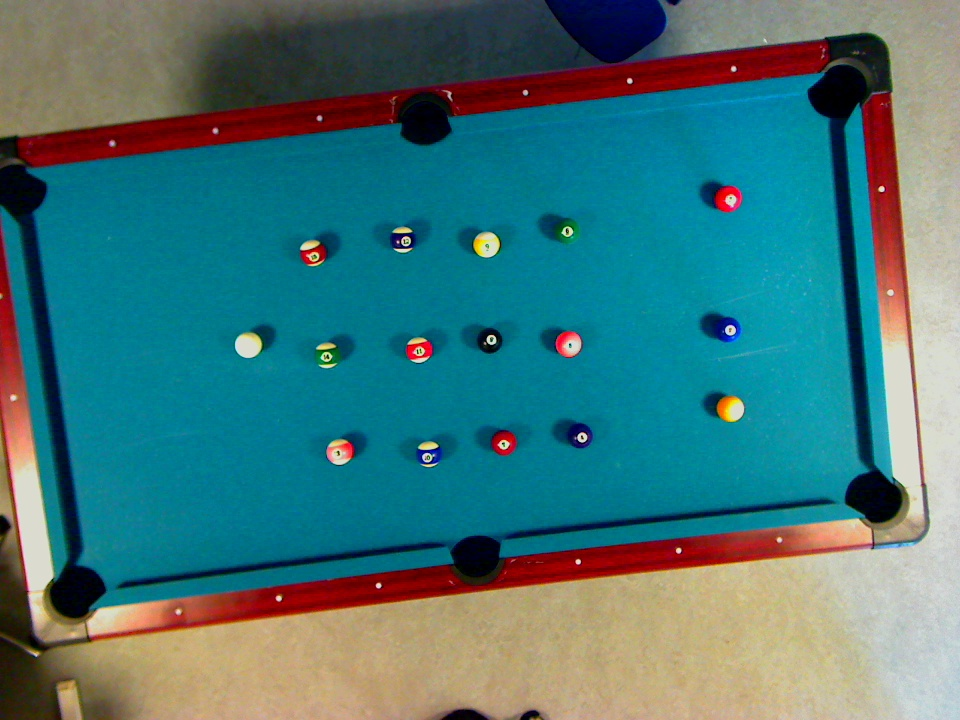
\includegraphics[width=0.5\textwidth]{images/default}
\end{center}
\caption{Default settings of camera parameters.}
\label{fig:defaultcamera}
\end{figure} 
	
As seen in image\ref{fig:defaultcamera} the ball towards the lower right corner is the solid yellow, but it seems to be half yellow and half white. This is due to overexposure and therefore saturation of the bright colors. The default camera settings is not the optimal settings for this project.\\	

A few examples of wrong settings can be seen in \ref{fig:wrongcamera}. They are divided into settings that only occur in software and settings that alter hardware parameters of the camera.

\begin{figure}[H]
\centering
\subfloat[Software: Wrong whitebalance.]
{
	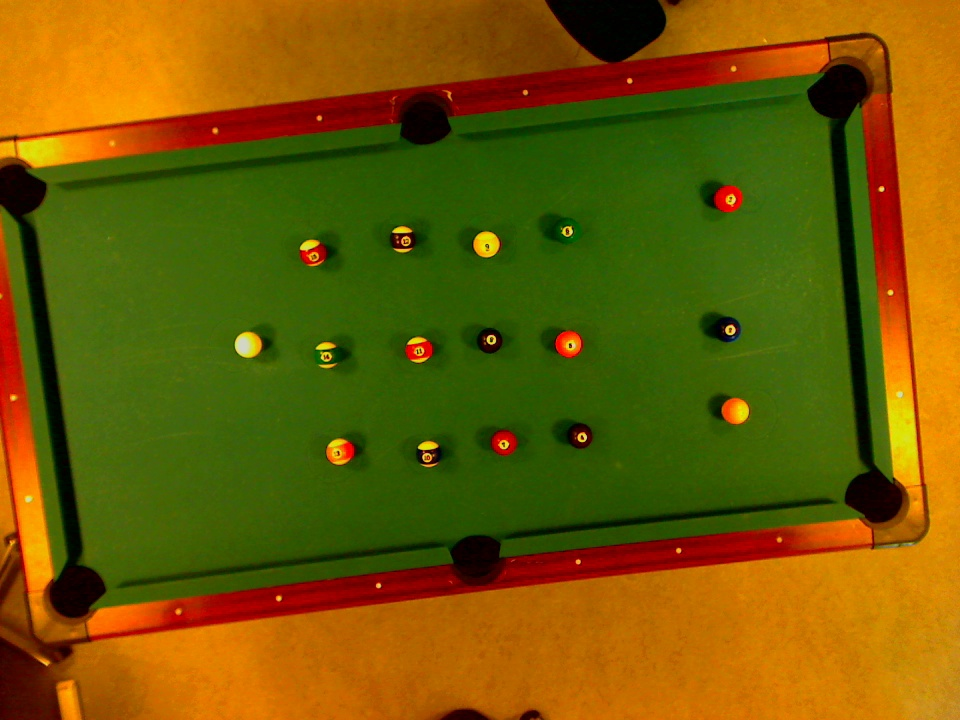
\includegraphics[width=0.4\textwidth]{images/badwhite}
}
\subfloat[Hardware: Extreme saturation.]
{
	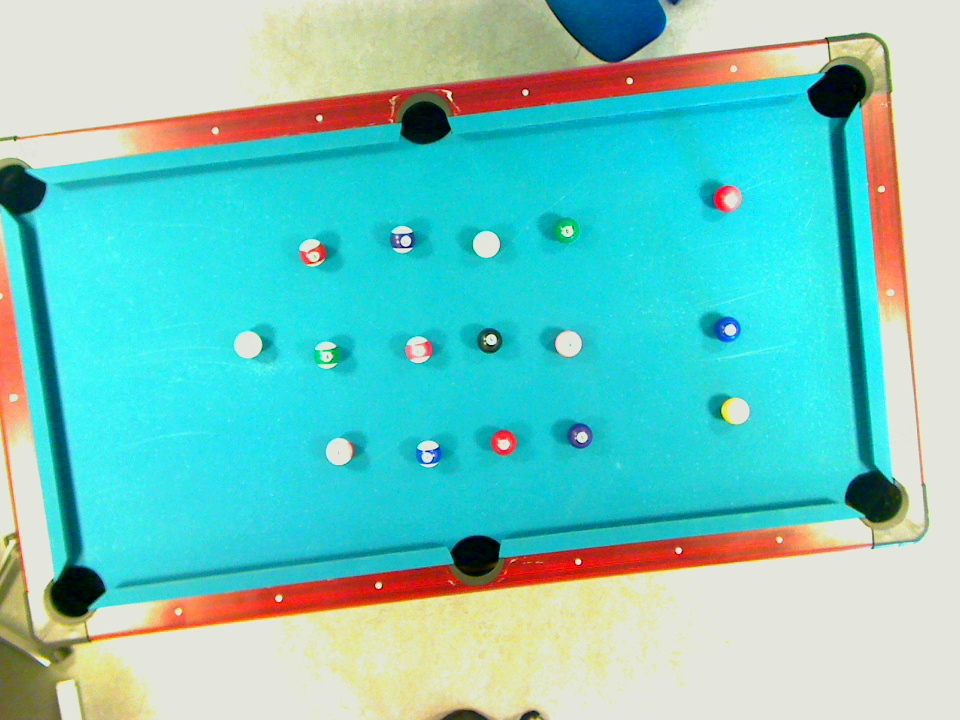
\includegraphics[width=0.4\textwidth]{images/overexposure}
}
\\
\subfloat[Hardware: Camera out of focus.]
{
	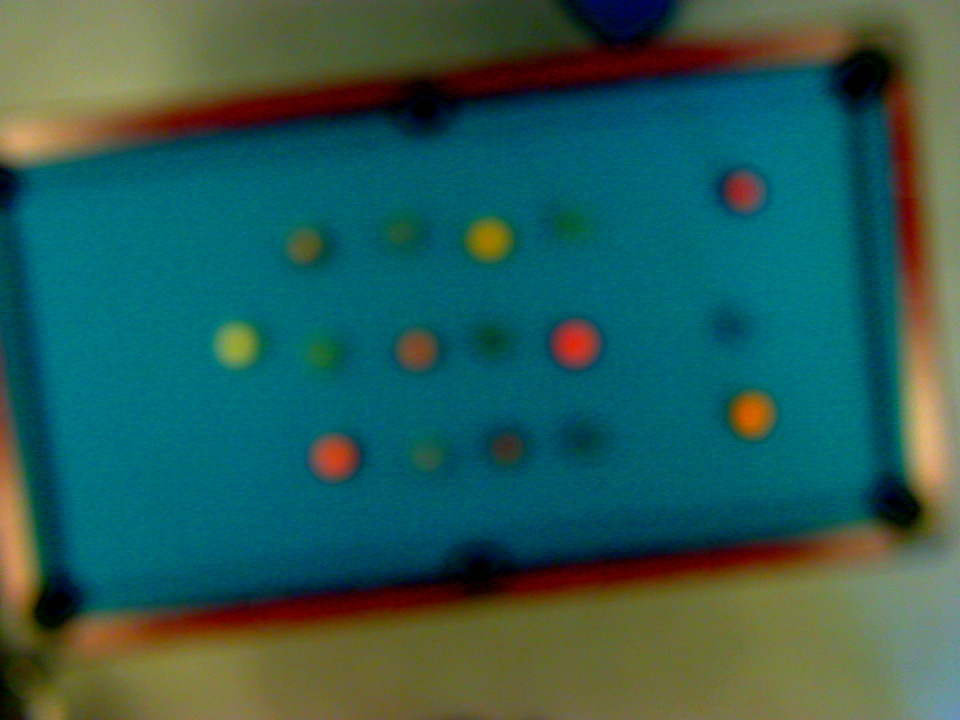
\includegraphics[width=0.4\textwidth]{images/nofocus}
}
\label{fig:wrongcamera}
\end{figure} 

The optimal settings can only be set using Logitech Quickcam software and manual input. The best image archived can be seen in \ref{fig:bestimgcamera}. The balls are easily distinguishable from each other and no saturation occurs.

\begin{figure}[H]
\begin{center}
\leavevmode
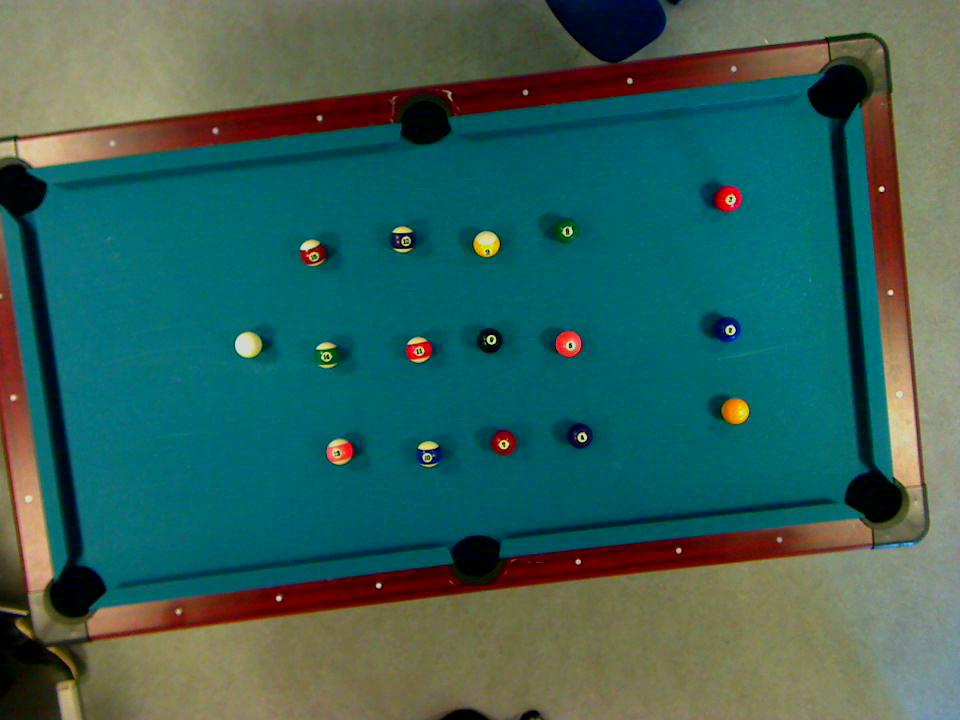
\includegraphics[width=0.5\textwidth]{images/good-from-program}
\end{center}
\caption{Image using optimal settings.}
\label{fig:bestimgcamera}
\end{figure} 

It is very important that the settings are set correctly to produce an optimal image. If saturation occurs the bright ball with solids colors could appears as ball with half color. If the color balance is not optimal the red, orange and brown balls might also look very alike.\\

The Logitech Quickcam software is not able to produce a high quality image of the pool table with default and auto settings.

